%#! platex thesis.tex

%======================================================================
% 章見出し
\chapter{文字認識に関する関連技術}
\label{cha:relate}
本章では,手書き文字認識技術として一般に用いられるオンライン文字認識とオフライン文字認識について説明する.さらに時系列データに対応した機械学習モデルである,再帰型ニューラルネットワークについて説明する.その後再帰型ニューラルネットワークを用いたオンライン文字認識の既存研究を述べ.遠隔医療での処方箋予測に向けたオンライン文字認識におけるデータ拡張に関する先行研究について述べる.
%----------------------------------------------------------------------

\section{手書き文字認識の種類}
\label{sec:rel_1}
手書き文字の認識は大きく2つに分けることができる.オフライン文字認識とオンライン文字認識である.オフライン文字認識は,文字の画像データにおいてそれぞれのピクセルが持つ情報を特徴量として文字を認識する技術であり,手書き文字は認識されるためにイメージスキャナやデジタルカメラによって読みとられる.
オンライン文字認識は手書き文字の$(x, y)$座標やスピード,筆圧などを特徴量として認識する技術で,通常タブレットなどに書き込まれた文字が認識される.

オフライン文字認識は画像認識技術であるため,文献\cite{yuan12:offline}のような畳み込みニューラルネットワーク(Convolutional Neural Network,以下CNN)を用いた文字認識が多く研究されている.利用可能な画像データもインターネット上に多く存在するが,実際に認識を行う際には手書きされた文字をスキャナやデジタルカメラなどで読み取る必要があるなどのデメリットもある.

一方でオンライン文字認識はIAM On-Line Handwriting Database\cite{iam},CASIA Chinese Handwriting Database\cite{liu11:casia}などのデータセットが存在するが,オフライン文字認識に比べると利用可能なデータは少ない.しかし認識時においてはタブレットなどのデバイスに書き込まれた手書き文字のデータが直接使われるため,オフライン文字認識と比べると手間が少ない.また,オンライン文字認識は筆順・筆圧・書き込みにかかる時間などの,オフライン文字認識では使うことができない情報を用いて認識を行うことができるなどのメリットがある.

本研究では,医者の手書き文字は筆記体が多く使われるため画像での認識は難しいと考えられること,実際に使用する際にはスキャンやデジタルカメラによる撮影を行わずリアルタイムでの認識を想定していることから,オンライン文字認識を用いて医者の手書き医療用語の認識を行う.

%----------------------------------------------------------------------
\section{再帰型ニューラルネットワーク}
再帰型ニューラルネットワーク(Recurrent Neural Network,以下RNN)とは中間層に戻り値のある,音声,動画,文章などの時系列データの扱いに優れているニューラルネットワークである.以下でRNNの構造と,再帰型ニューラルネットワークの一種であるLong Short-Term Memory(以下,LSTM)について説明する.本論文ではLSTMを用いて機械学習を行う.
\subsection{RNNの構造}
\label{ssec:rel_2}

\begin{figure}[tb]
 \begin{center}
  \resizebox{\columnwidth}{!}{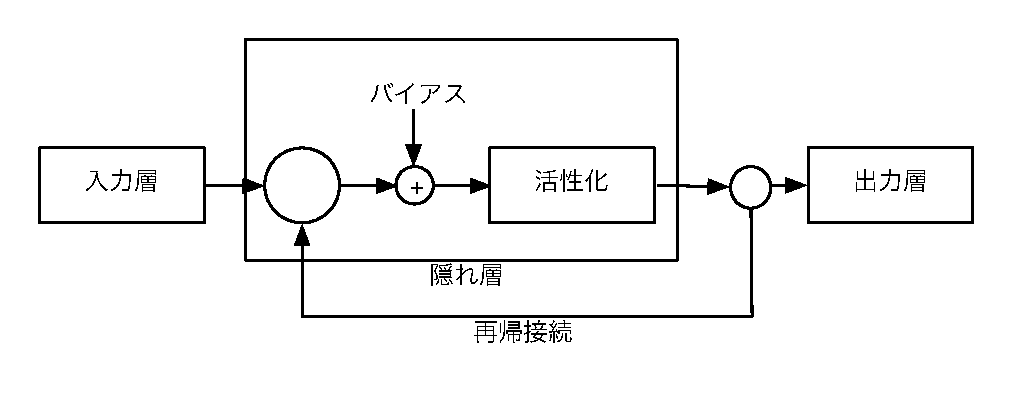
\includegraphics{img/rnn.eps}}
  \caption{RNNの構造}
  \label{rnn}
\end{center}
\end{figure}

\textbf{図~\ref{rnn}}に再帰型ニューラルネットワークの構造を示す.RNNは中間層のノードごとに戻り値があるため,現在入力されているデータより前のデータの影響を考慮して計算を行うことができる.そのためRNNは連続的な情報を保持したまま学習を行うことができる\cite{chakra16:bangla}.
式~\ref{eq:rnn-1}, 式~\ref{eq:rnn-2}に,RNNがそれぞれのノードにおいて行っている計算を入力値$x$と時間的順序$t$を用いて示す.
\begin{equation}
 H(t) = h(W_Hx(t) + W_{self}H(t-1) + b_H)
  \label{eq:rnn-1}
\end{equation}
\begin{equation}
 Y(t) = y(W_YH(t) + b_Y)
  \label{eq:rnn-2}
\end{equation}
ここにおいて$H(t)$は隠れ層の出力であり,$W_H$は隠れ層への入力の重み,$W_{self}$は戻り値の重み,$b_H$は隠れ層へのバイアス,$Y(t)$はネットワークの出力,$W_Y$は隠れ層の出力の重み,$b_Y$は出力へのバイアス,$y()$と$h()$はそれぞれ出力層と隠れ層の活性化関数である.式より,隠れ層の出力は隠れ層への入力$x(t)$だけでなく,隠れ層からの1つ前の出力$H(t-1)$の影響も受けていることがわかる.したがってネットワークの出力$Y(t)$は$x(t)$と$x(t-1)$の影響を受けていると言える.この計算は最初をのぞいた全ての入力において行われている.

\begin{figure}[tb]
 \begin{center}
  \resizebox{\columnwidth}{!}{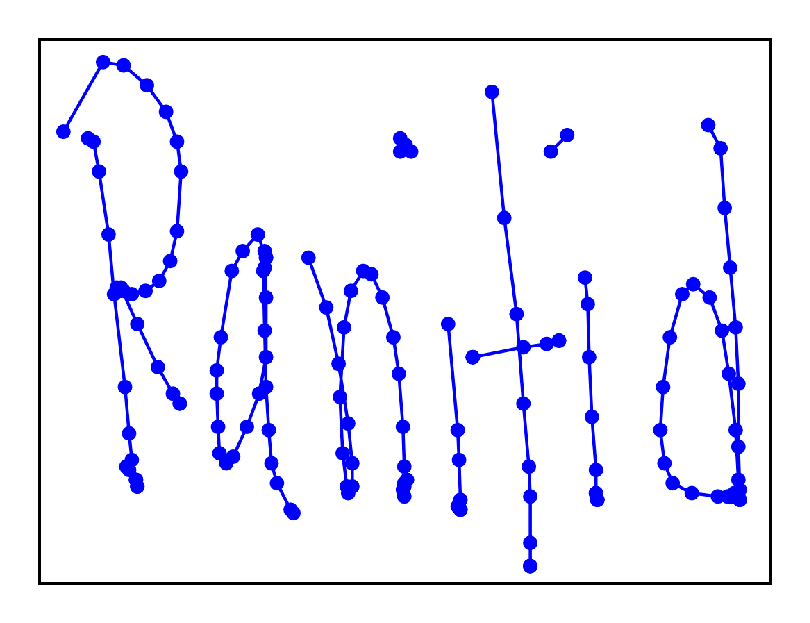
\includegraphics{img/ranitid.eps}}
  \caption{文字を点で表した図}
  \label{original}
\end{center}
\end{figure}

\textbf{図~\ref{original}}に認識する手書き文字の例を示す.このように,手書き文字は検出された座標が時間的順序に従って並んだものであると言える.オフライン文字認識では,手書き文字を画像データとして捉えるため,点の時間的順序を考慮に入れずに認識を行う.RNNの入力に連続した手書き文字の点データを用いることで,オンライン文字認識ではその時間的順序を考慮に入れて認識を行うことができる.

しかし,実際にRNNで出力に反映できる過去の入力情報は短く,時系列10ステップ分程度であると言われている\cite{okatani15:deep_learning}.

\subsection{LSTM}
\label{ssec:lstm}

\begin{figure}[tb]
 \begin{center}
  \resizebox{\columnwidth}{!}{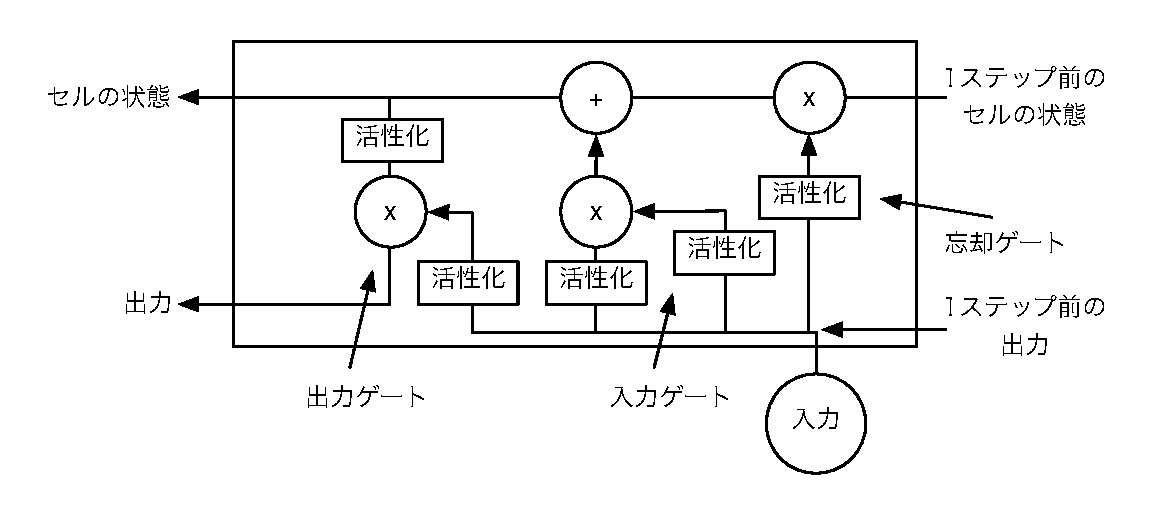
\includegraphics{img/lstm.eps}}
  \caption{LSTMブロックの構造}
  \label{lstm}
\end{center}
\end{figure}

\textbf{図~\ref{lstm}}にLSTMブロックの構造を示す.LSTMはRNNよりも長期にわたる記憶を実現するための方法のひとつで,RNNの隠れ層の各ユニットをLSTMブロックに置き換えたものである.RNNのユニットと異なり,LSTMブロックは記憶を持ったセルの構造をしている.ゲートと呼ばれる特殊な構造がセルに情報を与えるかセルの情報を除去するかを決める.

忘却ゲートがセル内の情報をリセットし,入力ゲートは,入力が現在のセルにどれだけ影響を与えるか決める.出力ゲートは出力が残りのネットワークにどれだけの影響を与えるか決める.この方法によってLSTMはより長い時系列データにおける再帰型ニューラルネットワークの利用を可能にしている.

%----------------------------------------------------------------------
\section{関連研究}
\label{sec:rel_3}
ここではLSTMを用いたオンライン文字認識の既存研究と,文字認識におけるデータ拡張に関する既存研究について述べる.

\subsection{直線データとBidirectionalLSTMを用いた中国語認識システム\cite{zhang18:drawing}}
\label{ssec:drawing}
文献\cite{zhang18:drawing}では中国語手書き漢字の座標データの中から,直線上の点や近接する点など,取り除いても文字として成り立つ点を除去したのち直線データに変換し,BidirectionalLSTMを用いて認識を行っている.BidirectionalLSTMについては\ref{sec:m_learning}節で述べる.点の除去を行うことで入力データを簡易化し,さらに直線データへの変更を行うことで連続する点同士の関係性(点同士の距離,次の点への角度,同一字画上にあるかなど)を特徴量として抽出することができる.機械学習モデルにはBidirectionalLSTMを用いることで,入力されているより過去の座標の情報だけでなく未来の座標の情報も考慮に入れた学習を行うことができる.

\subsection{dropStroke手法を用いたデータ拡張と筆者同定システム\cite{yang15:dropstroke}}
文献\cite{yang15:dropstroke}では中国語手書き漢字において,座標の時系列データから一部のストロークを除去する処理を複数回繰り返すことでデータ拡張を行い, CNN を用いたオフライン認識で筆者の同定を行っている.文字としては不完全なデータになるが筆者の特徴を大きく変えることにはならず,100\% に近い精度での筆者同定を可能にしている.ただし,ストロークを除去することで異なる文字・単語になってしまう可能性があり,本論文の目的とする単語認識においてこの手法は適切であるとは言えない.同著者からは,筆者同定のためのデータ拡張として dropSegment 手法というものも提案されているが\cite{yang16:dropsegment},これも異なる文字・単語に変わってしまう可能性があり,単語認識に適切であるとは言えない.

%================================================================================================
\section{先行研究}
\label{sec:rel_4}
遠隔医療システムにおける処方箋予測に向けた手書き医療用語認識に関する研究\cite{takahashi}では,処方箋の予測に向けたシステムの初期研究として,再帰型ニューラルネットワークの一種であるBidirectionalLSTMを用いたオンライン手書き医療用語認識手法の提案を行っている.また様々な手書き文字に対応するため,文字認識では多様な提供者から大量のデータを得る必要がある.しかし,十分なデータ量を確保するためには非常に多くの労力と時間を要する.そこで筆者はオンライン手書き文字のデータ拡張手法として,ストロークの回転と平行移動によってデータ量を水増しするStroke Rotation and Parallel-shift(SRP)手法を提案している.
手書き文字データは,文献\cite{zhang18:drawing}を用いてデータの簡易化,特徴量の抽出を行っている.また文献\cite{takahashi}ではPortable Health Clinicにおける過去の処方箋データから頻出する単語を座標の時系列データとして収集している.収集した15991語のデータを用いて,SRP手法でデータ拡張を行った後にBidirectionalLSTMで学習を行った結果,480語のクラスにおいて89.5\%の精度で単語を認識している.この結果はデータ拡張を行わなかった場合の認識精度と比べて16.1\%高い.
しかしSRP手法において回転の大きさ,平行移動の大きさは筆者が文字の形を崩さないと判断できる範囲で設定しているため,データを高倍率で拡張した場合に同じような値を用いてしまい,拡張後に同じようなデータが増えて学習精度が低くなる原因になってしまう.そのため,この用語認識は学習の際にランダムに設定された回転の大きさと平行移動の大きさの組み合わせにより,認識精度にばらつきが出てしまうという問題がある.

% 以下はRefTeX用
%%% Local Variables:
%%% mode: yatex
%%% TeX-master: "thesis"
%%% End:
